\begin{figure} [t]
    \vspace{-6pt}
    \centering
    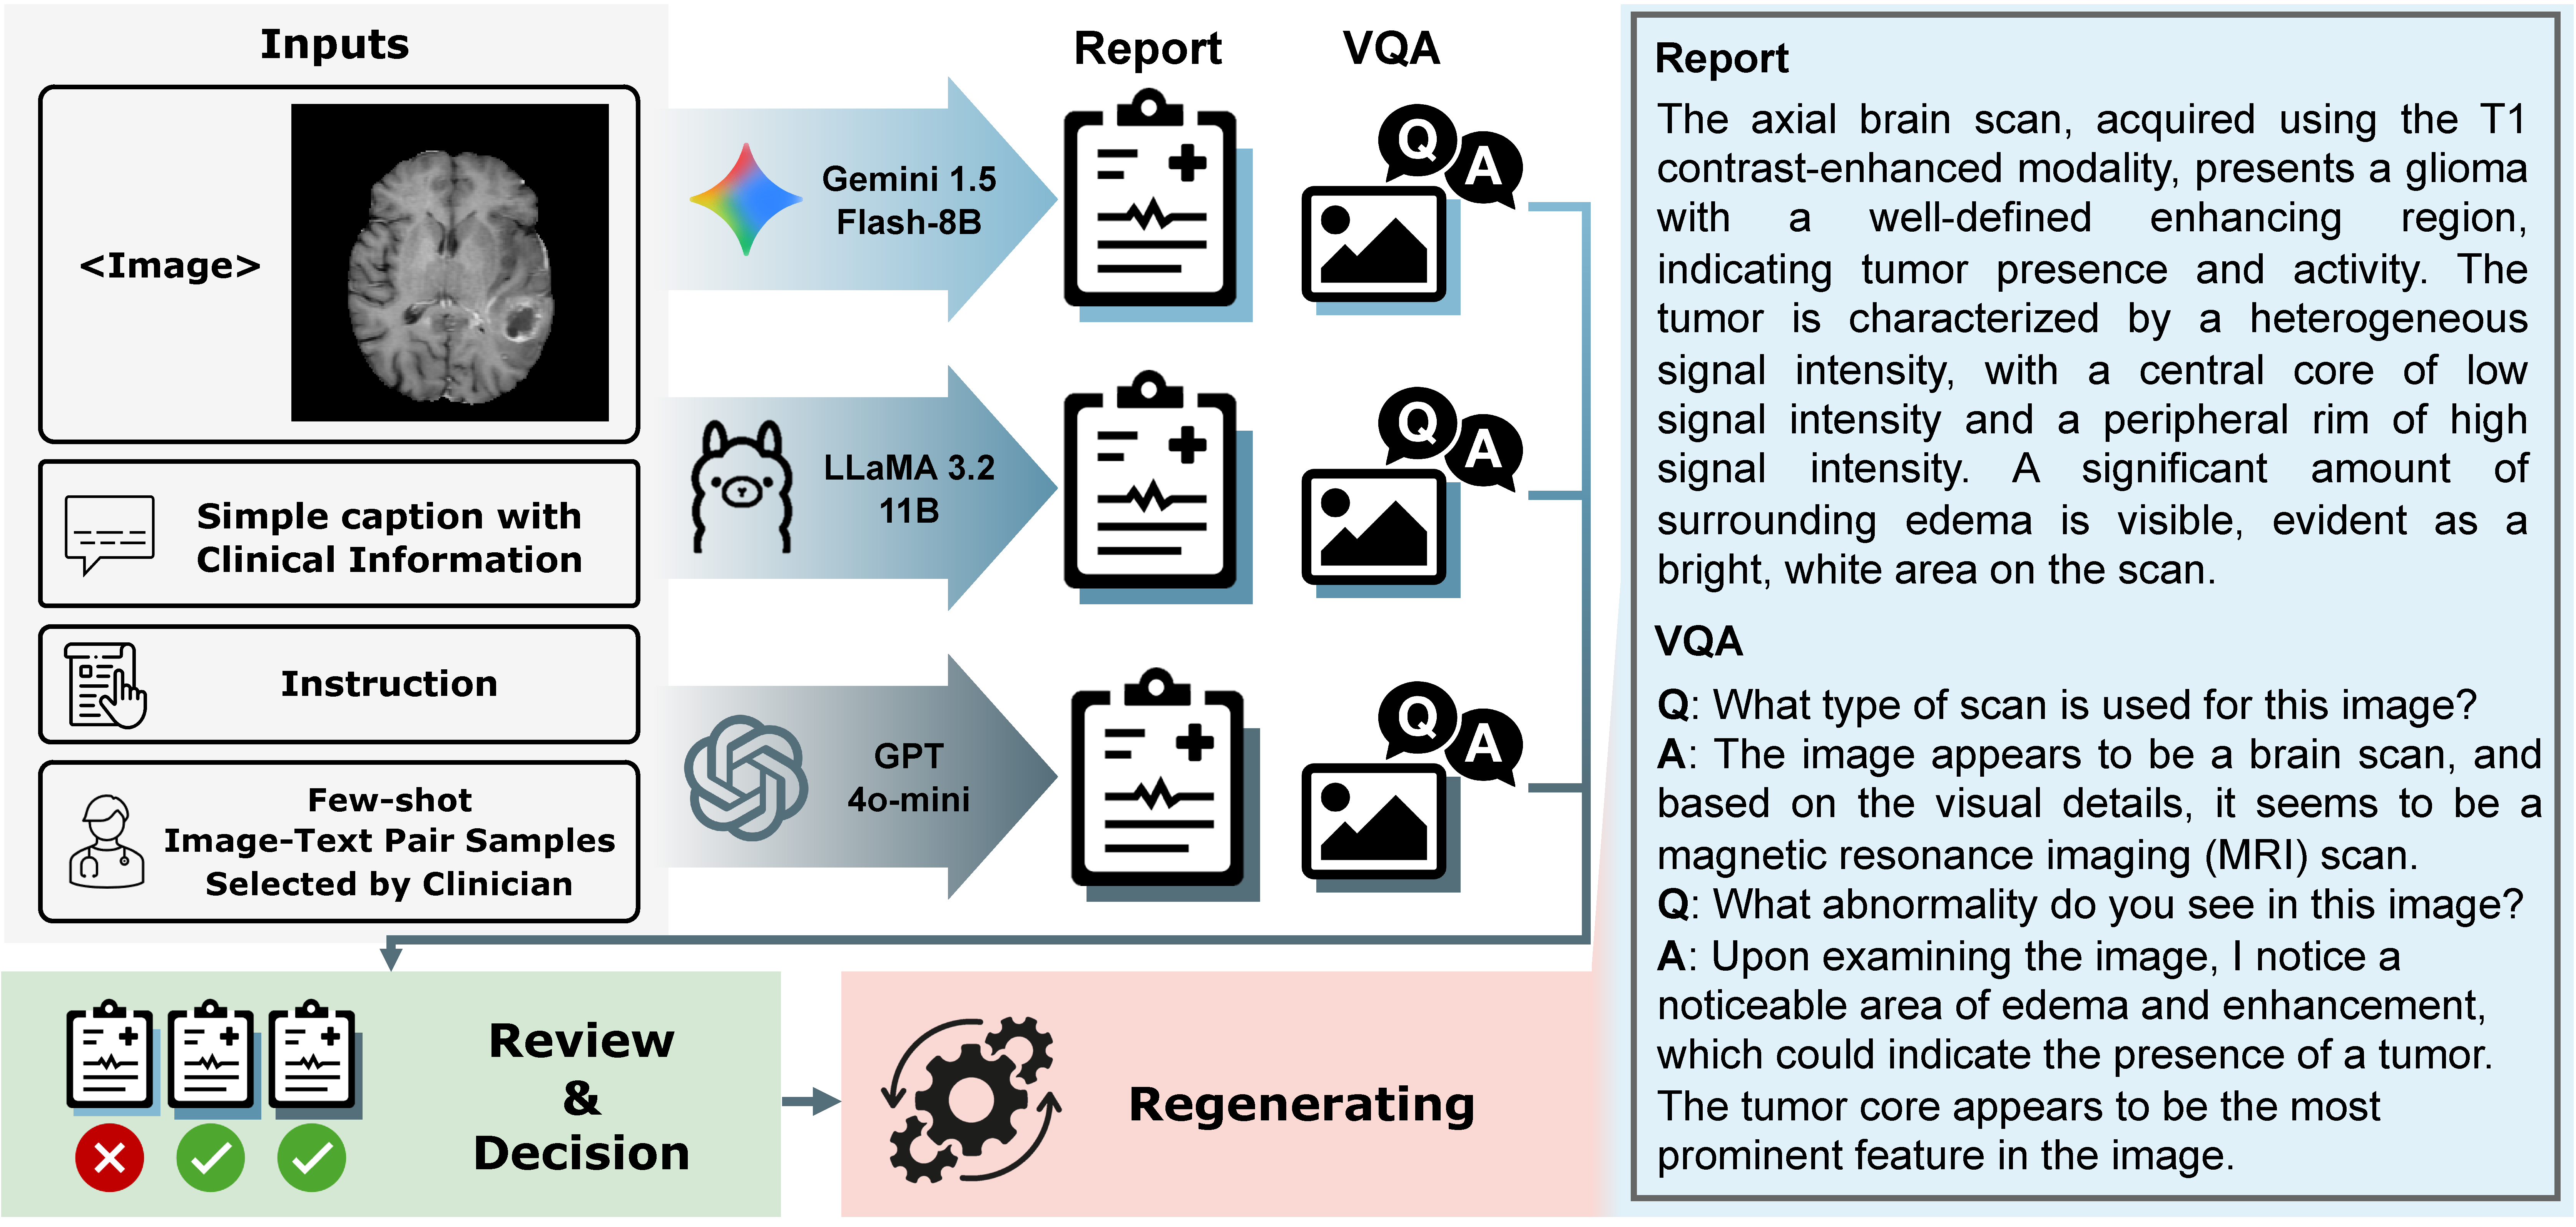
\includegraphics[width=0.99\textwidth]{figs/fig2.pdf}
    \centering
    \vspace{-3pt}
    \caption{\textbf{Text data generation with LLMs on a dataset with only images.} Images and captions are processed by LLMs with strict predefined instructions and few-shot samples selected by clinicians to generate reports and VQA results. The output of each model is accepted or rejected using GPT 4o and the final report and VQA are regenerated based on this feedback.}
    \vspace{-6pt}
    \label{fig2}
\end{figure}

\begin{figure*} [t]
    \vspace{-6pt}
    \centering
    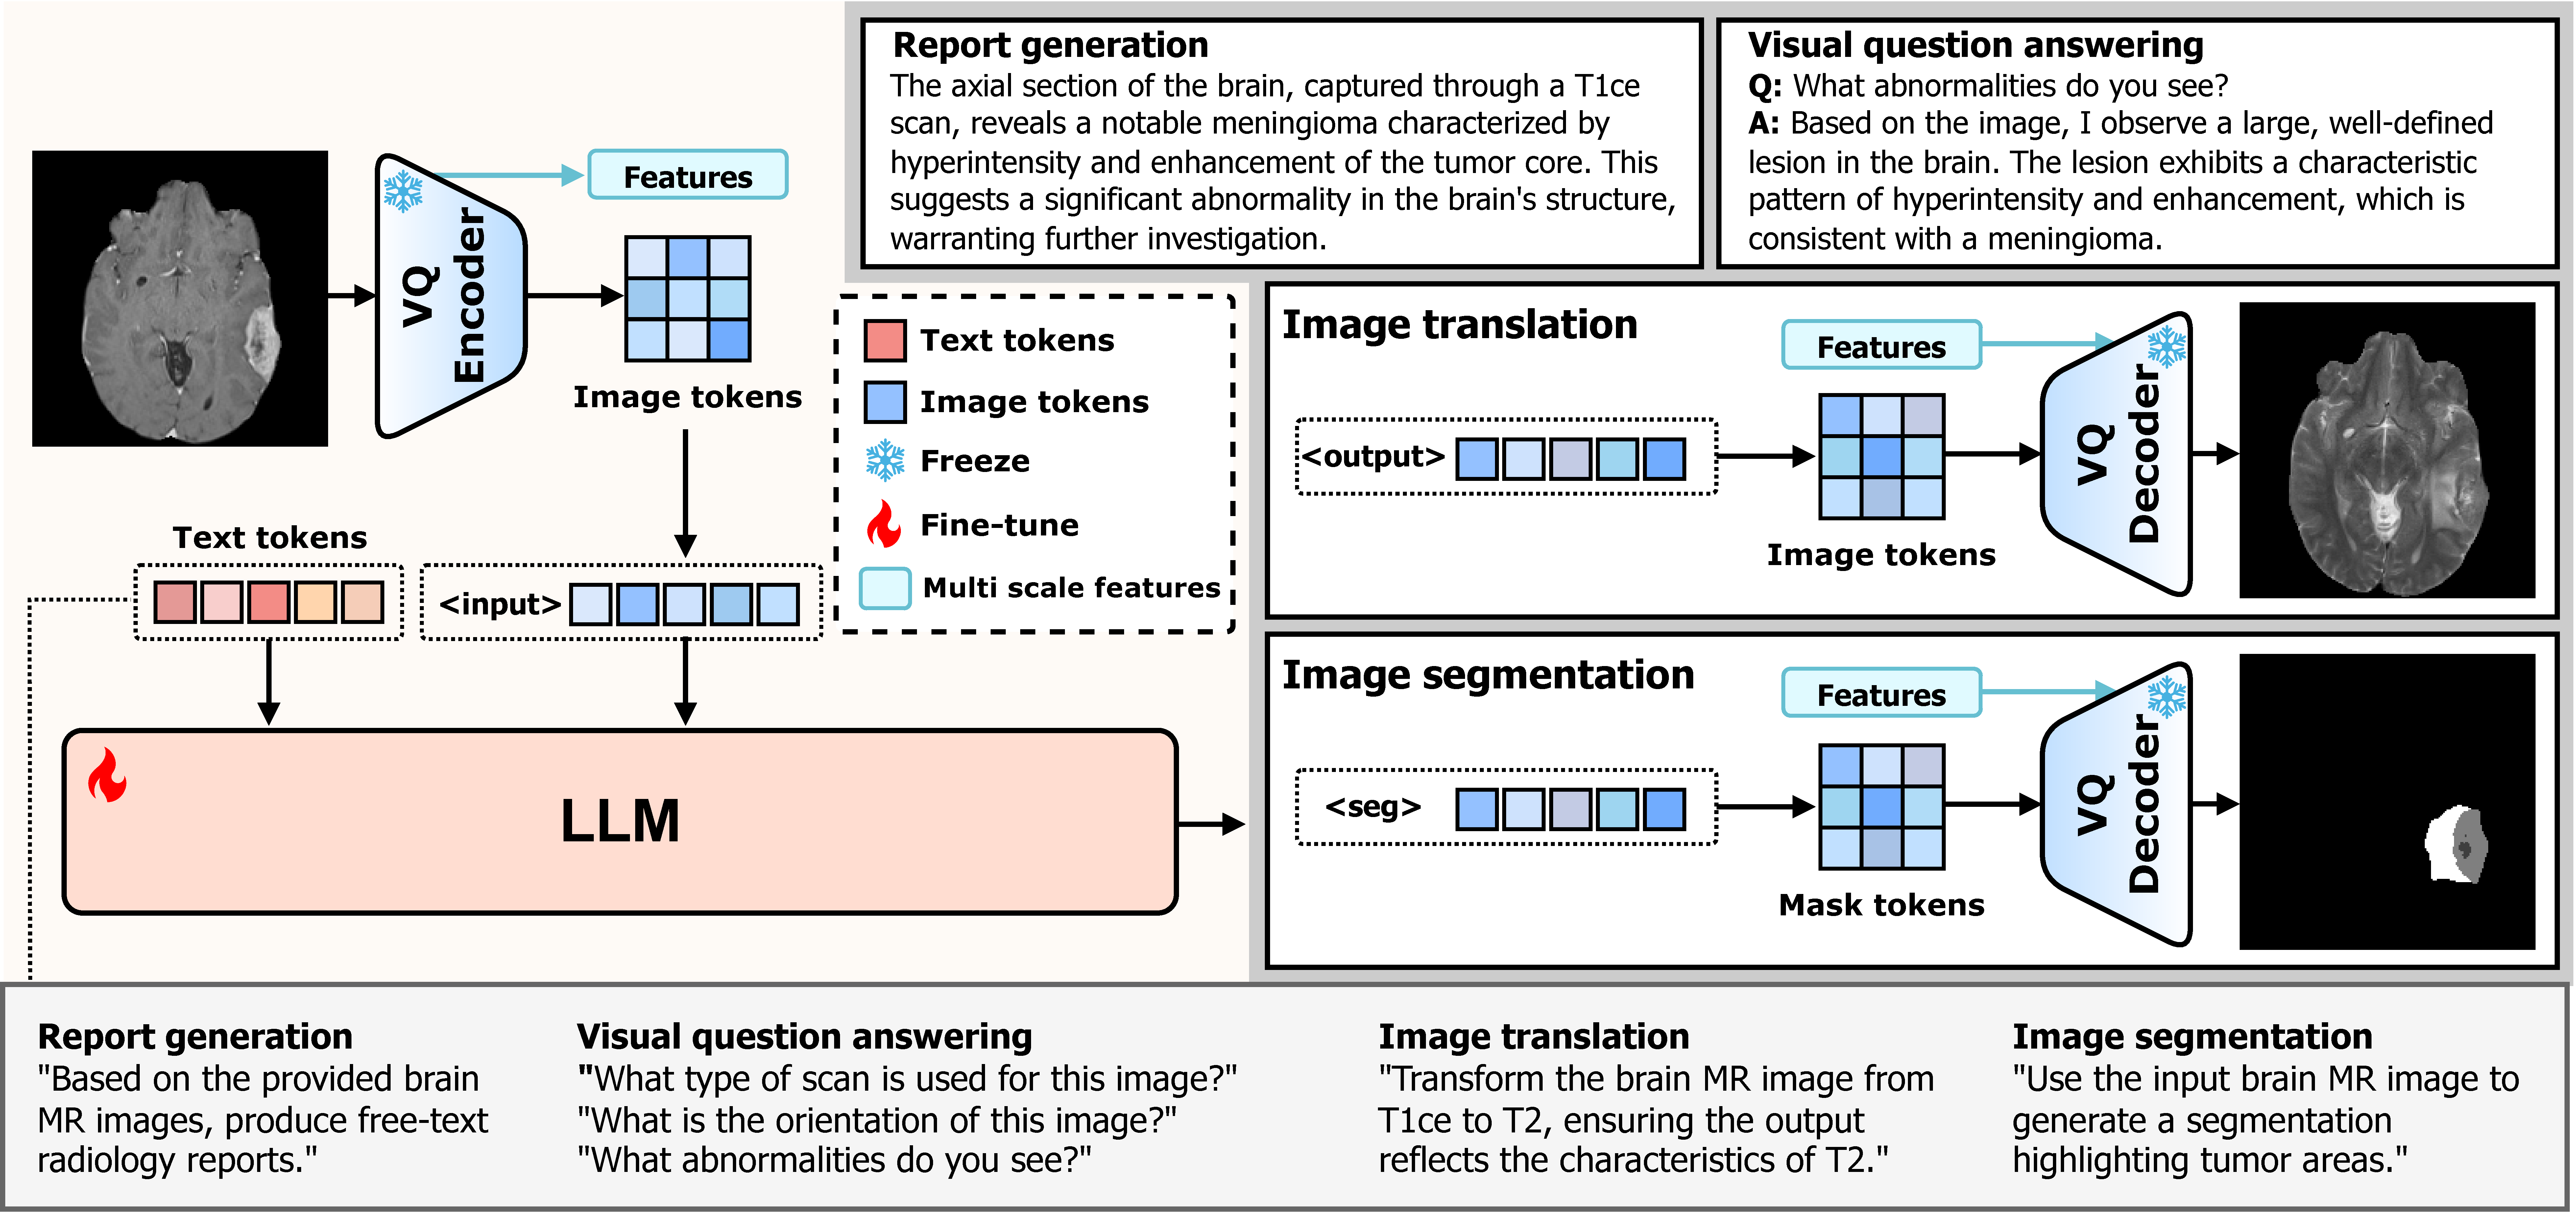
\includegraphics[width=0.99\textwidth]{figs/fig3.pdf}
    \vspace{-3pt}
    \caption{\textbf{Instruction tuning pipeline.} Both text and images are tokenized and fed into the LLM, which can generate either text or image tokens as output. The LLM's vocabulary is extended to include image tokens in addition to text tokens. The instruction is provided to the LLM as text tokens. The image is converted into quantized tokens using a VQ encoder and fed into the LLM along with an \texttt{<input>} token. These image tokens are added to the LLM's vocabulary as discrete values, similar to text tokens. For image translation, the output is generated with an \texttt{<output>} token, while for segmentation, the output is generated with a \texttt{<seg>} token.}
    \vspace{-6pt}
    \label{fig3}
\end{figure*}

\section{Related Work}
\noindent \textbf{Language Models for Medicine.} 
LLMs pretrained on large amounts of text data have made remarkable progress and have been applied to various downstream tasks such as translation, question answering, and text generation \cite{achiam2023gpt,team2023gemini,touvron2023llama,touvron2023llama2openfoundation,grattafiori2024llama3herdmodels,ra2025enhancing}. LLaVA \cite{liu2023visual} successfully integrates image and text information by generating VQA data using image and object location information and applying instruction tuning, even when image-text pairs are limited. In the medical domain, models such as LLaVA-Med \cite{li2024llava} and BioMed-VITAL \cite{cui2024biomedical} have demonstrated the potential to generate captions for medical images and assist in explanation and diagnosis. In addition, medical multimodal LLMs have begun to emerge recently \cite{moor2023med,thawkar2023xraygpt,chaves2024towards,lee2025cxr}. Specifically, LLM-CXR \cite{lee2024llmcxr} proposes a unified model that supports both image-to-text and text-to-image functions for chest X-rays, highlighting its versatility. However, most of these studies have focused on CXR datasets, where paired image-text data is available, while similar research on brain MRI is rare.

\vspace{3pt}
\noindent \textbf{Image-to-Image Tasks with Language Models.}
In image segmentation, several methods combine language models with pretrained CLIP \cite{radford2021learning} or introduce a \texttt{<SEG>} token into LLaVA \cite{liu2023visual}. M3D \cite{bai2024m3d} integrates medical images into large language models such as LLaMA2 \cite{touvron2023llama2openfoundation} to perform both segmentation and text generation tasks.
In image translation, methods that synthesize images by incorporating natural language descriptions using pretrained CLIP have been actively studied. DiffuseIT \cite{kwon2023diffusionbased} integrates text information directly into the noise reduction steps of the diffusion process so that the generated image follows the text prompt. ControlNet \cite{zhang2023adding} leverages Stable Diffusion and adds an extra branch that uses a control image and text prompts to guide image synthesis. However, these approaches are task-specific models designed for image synthesis utilizing embeddings of language models. 